\documentclass[11pt]{charter}
%%%% aqui para el paquete
\usepackage{pdflscape} % paquete para girar la hoja
\usepackage[most]{tcolorbox} % paquete para poner borde a imagen
\usepackage{rotating} % para rotar tabla


% El títulos de la memoria, se usa en la carátula y se puede usar el cualquier lugar del documento con el comando \ttitle
\titulo{Sistema de control y monitoreo para viviendas y edificios} 

% Nombre del posgrado, se usa en la carátula y se puede usar el cualquier lugar del documento con el comando \degreename
%\posgrado{Carrera de Especialización en Sistemas Embebidos} 
\posgrado{Carrera de Especialización en Internet de las Cosas} 
%\posgrado{Carrera de Especialización en Intelegencia Artificial}
%\posgrado{Maestría en Sistemas Embebidos} 
%\posgrado{Maestría en Internet de las cosas}

% Tu nombre, se puede usar el cualquier lugar del documento con el comando \authorname
\autor{Daniel Iván Cruz Flores} 

% El nombre del director y co-director, se puede usar el cualquier lugar del documento con el comando \supname y \cosupname y \pertesupname y \pertecosupname
\director{Mg. Ing. Matías Alvarez}
\pertenenciaDirector{FIUBA} 
% FIXME:NO IMPLEMENTADO EL CODIRECTOR ni su pertenencia
\codirector{} % si queda vacio no se deberíá incluir 
\pertenenciaCoDirector{}

% Nombre del cliente, quien va a aprobar los resultados del proyecto, se puede usar con el comando \clientename y \empclientename
\cliente{ Gabriela de la Cruz}
\empresaCliente{ICF Network}

% Nombre y pertenencia de los jurados, se pueden usar el cualquier lugar del documento con el comando \jurunoname, \jurdosname y \jurtresname y \perteunoname, \pertedosname y \pertetresname.
\juradoUno{Nombre y Apellido (1)}
\pertenenciaJurUno{pertenencia (1)} 
\juradoDos{Nombre y Apellido (2)}
\pertenenciaJurDos{pertenencia (2)}
\juradoTres{Nombre y Apellido (3)}
\pertenenciaJurTres{pertenencia (3)}
 
\fechaINICIO{25 de agosto de 2020}		%Fecha de inicio de la cursada de GdP \fechaInicioName
\fechaFINALPlanificacion{13 de octubre de 2020} 	%Fecha de final de cursada de GdP
\fechaFINALTrabajo{31 de agosto de 2021}		%Fecha de defensa pública del trabajo final


\begin{document}

\maketitle
\thispagestyle{empty}
\pagebreak


\thispagestyle{empty}
{\setlength{\parskip}{0pt}
\tableofcontents{}
}
\pagebreak


\section{Registros de cambios}
\label{sec:registro}


\begin{table}[ht]
\label{tab:registro}
\centering
\begin{tabularx}{\linewidth}{@{}|c|X|c|@{}}
\hline
\rowcolor[HTML]{C0C0C0} 
Revisión & \multicolumn{1}{c|}{\cellcolor[HTML]{C0C0C0}Detalles de los cambios realizados} & Fecha      \\ \hline
1.0      & Creación del documento                                          & 27/06/2020 \\ \hline
1.1      & Entrega del documento hasta el punto 6 \newline
			(sin incluir canvas e historias de usuarios)            & 07/09/2020 \\ \hline
1.2      & Entrega del documento completo hasta el punto 6          & 15/09/2020 \\ \hline
1.3      & Entrega del documento hasta el punto 11  & 22/09/2020 \\ \hline
1.4      & Entrega final hasta el punto 17 \newline
			(documento completo)
 & 29/09/2020 \\ \hline
\end{tabularx}
\end{table}

\pagebreak



\section{Acta de constitución del proyecto}
\label{sec:acta}

\begin{flushright}
Buenos Aires, \fechaInicioName
\end{flushright}

\vspace{2cm}

Por medio de la presente se acuerda con el Ing. \authorname\hspace{1px} que su Trabajo Final de la \degreename\hspace{1px} se titulará ``\ttitle'', consistirá esencialmente en el prototipo preliminar de un sistema capaz de controlar y monitorear viviendas u otros ambientes mediante el protocolo MQTT para brindar una gestión inteligente y tendrá un presupuesto preliminar estimado de 610 hs de trabajo y S/2979.75, con fecha de inicio \fechaInicioName\hspace{1px} y fecha de presentación pública \fechaFinalName.

Se adjunta a esta acta la planificación inicial.

\vfill

% Esta parte se construye sola con la información que hayan cargado en el preámbulo del documento y no debe modificarla
\begin{table}[ht]
\centering
\begin{tabular}{ccc}
\begin{tabular}[c]{@{}c@{}}Ariel Lutenberg \\ Director posgrado FIUBA\end{tabular} & \hspace{2cm} & \begin{tabular}[c]{@{}c@{}}\clientename \\ \empclientename \end{tabular} \vspace{2.5cm} \\ 
\multicolumn{3}{c}{\begin{tabular}[c]{@{}c@{}} \supname \\ Director del Trabajo Final\end{tabular}} \vspace{2.5cm} \\
%\begin{tabular}[c]{@{}c@{}}\jurunoname \\ Jurado del Trabajo Final\end{tabular}     &  & \begin{tabular}[c]{@{}c@{}}\jurdosname\\ Jurado del Trabajo Final\end{tabular}  \vspace{2.5cm}  \\
%\multicolumn{3}{c}{\begin{tabular}[c]{@{}c@{}} \jurtresname\\ Jurado del Trabajo Final\end{tabular}} \vspace{.5cm}                                                                     
\end{tabular}
\end{table}




\section{Descripción técnica-conceptual del proyecto a realizar}
\label{sec:descripcion}
La tecnología de automatización orientada a viviendas y lugares de trabajo está tomando cada vez mayor relevancia en nuestras vidas, aunque existen muchas soluciones que ofrecen dotar de tecnología a ciertos elementos en un ambiente, su principal desventaja es que casi siempre la recolección de datos se realiza con sensores que dependen de una conexión a Internet para enviar sus valores a un servidor central para su gestión. Esta forma de trabajo permite la facilidad de uso pero con la desventaja de que la gestión funciona solo si existe conexión a Internet, además los sensores más comerciales están destinados a un uso individual con su propia aplicación móvil, complicando la necesidad de tener una única solución centralizada ante el uso de múltiples sensores.

El presente proyecto se destaca especialmente por centralizar y unificar resultados de la red de sensores en un sistema web principal de monitoreo y control sin depender de la conexión a Internet para su funcionamiento. Para lograr esta tarea se trabajará con la recolección de datos de sensores ubicados en distintos puntos de estudio de una vivienda o ambiente conectados a una red local dedicada. Cada una de las lecturas de los sensores serán enviadas a una unidad central local mediante el protocolo MQTT por vía inalámbrica, dejando la dependencia del Internet solo para los accesos remotos. El módulo central local contará con la función para replicar los valores recolectados hacia un servicio en la nube, tarea que se realizará mientras tenga conexión a Internet.

Las funciones principales a implementar están orientados a confort (control de ventiladores y luces) y consumo energético (consumo de energía de tv, refrigerador y ventiladores). En la Figura \ref{fig:diagBloques} se presenta el diagrama de bloques del sistema. 

El sistema a desarrollar contará de dos formas de acceso: la primera es vía red local y la segunda vía Internet desde cualquier dispositivo mediante un navegador.

%\vspace{20px}

\begin{figure}[htpb]
\centering 
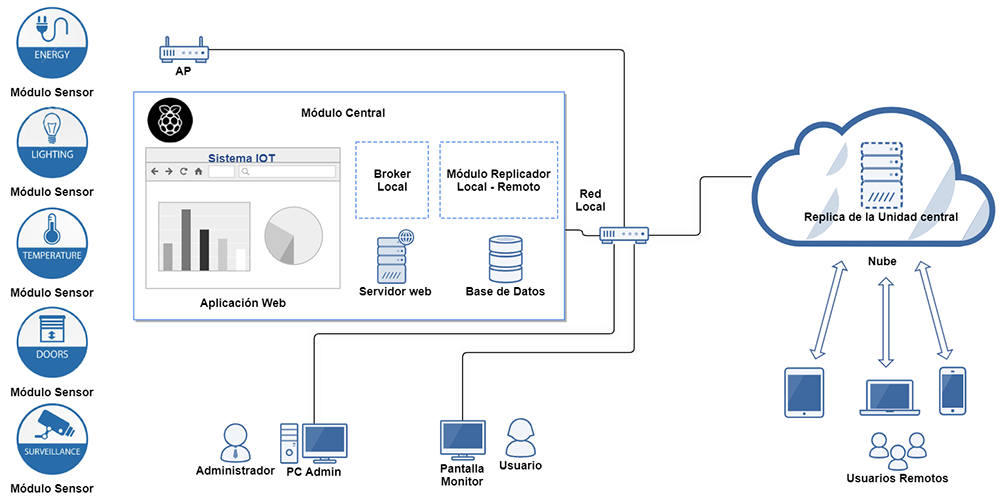
\includegraphics[width=0.73\textwidth]{./Figuras/diagBloques.png}
\caption{Diagrama en bloques del sistema}
\label{fig:diagBloques}
\end{figure}

%\vspace{20px}

A continuación se detalla brevemente cada componente que comprende el presente proyecto.

a) MÓDULO PRINCIPAL: unidad central local.
\begin{itemize}
\item Hardware: raspberry Pi 4.
\item Sistema operativo: raspbian.
\item Servidor web: apache.
\item Base de datos: MySql.
\item Lenguajes backend: python, php 7.
\item Lenguajes frontend: html5, css – bootstrap 4 y javascript.
\item Broker MQTT: eclipse mosquitto.
\item Interfaz - Monitor: pantalla monitor/pantalla touch.
\item Importancia: este es el módulo principal y el más complejo a desarrollar, es donde se podrá observar un dashboard (resumen) del sistema de control y monitoreo para su acceso en red local. La interfaz gráfica mostrará gráficos estadísticos así como un historial de las lecturas de los sensores y sus estados.
\end{itemize}

b) MÓDULO RÉPLICA: unidad remota.
\begin{itemize}
\item Servidor web: apache (hosting o nube).
\item Base de datos: MySql.
\item Lenguajes backend: php 7.
\item Lenguajes frontEnd: html5 y css – bootstrap 4 y javascript.
\item Importancia: este es una réplica del módulo principal en la nube donde se podrá observar un dashboard del sistema de control y monitoreo para el acceso remoto.
\end{itemize}


c) MÓDULO CONSUMO: para medir consumo energético.
\begin{itemize}
\item Hardware base: nodeMCU esp8266.
\item Lenguaje: arduino.
\item Protocolo de comunicación: MQTT.
\item Sensor: corriente AC max 100A no invasivo.
\item Medio transmisión: wireless.
\item Cantidad: 1.
\item Objetos de estudio: tv y refrigerador.
\item Importancia: este módulo permite recoger muestras del valor del consumo diario para poder almacenarlos en la base de datos en el módulo principal. A su vez, sirve para estimar costos de consumo mensual; información relevante para el usuario porque permitirá saber el consumo detallado de los dispositivos de estudio.
\end{itemize}

d) MÓDULO TEMPERATURA: para medir temperatura - confort.
\begin{itemize}
\item Hardware base: nodeMCU esp8266.
\item Lenguaje: arduino
\item Protocolo de comunicación: MQTT.
\item Sensor: temperatura ambiente.
\item Medio de transmisión: wireless.
\item Cantidad: 1.
\item Objetos de estudio: sala y una oficina.
\item Importancia: este módulo permite recoger muestras del valor de la temperatura en determinados ambientes de estudio, dichos valores pueden ser almacenados y usados para estudio de patrones de variación de temperatura por horarios.
\end{itemize}

e) MÓDULO ACTUADOR: para control actuador - confort.
\begin{itemize}
\item Hardware base: nodeMCU esp8266.
\item Lenguaje: arduino.
\item Protocolo de comunicación: MQTT.
\item Actuador: relay de un canal.
\item Medio de transmisión: wireless.
\item Cantidad: 1.
\item Objetos de estudio: control de ventiladores (según datos del módulo temperatura).
\item Importancia: este actuador es un módulo complementario del "módulo temperatura"; permitirá saber el historial de uso y demanda de uso de ventiladores; patrones que pueden ser tema de estudio relacionado al consumo en aplicaciones futuras.
\end{itemize}

f) MÓDULO INTELIGENTE: para medir y controlar de forma inteligente - confort y salud.
\begin{itemize}
\item Hardware base: raspberry Pi/esp32 cam/Otro.
\item Lenguaje: arduino y python.
\item Protocolo de comunicación: MQTT.
\item Actuador: real-time face recognition.
\item Sensor: lectura de temperatura corporal.
\item Medio de transmisión: wireless.
\item Cantidad: 1.
\item Objeto de estudio: seguimiento de posibles casos de fiebre.
\item Importancia: este módulo es el segundo módulo complejo a desarrollar por la forma a implementar para la identificación del individuo y la relación de lecturas de temperatura. Con los datos almacenados se puede usar para un estudio de patrones respecto de fechas y estaciones de fiebre. Por el momento se considera en este módulo el tema: "temperatura corporal", pero para trabajos futuros se puede extender las funcionalidades.
\end{itemize}

\section{Modelo canvas del negocio del proyecto}

Los elementos que describen la propuesta de negocio y los distintos puntos más importantes respecto a la orientación de mercado se muestra en el modelo canvas. En la Figura \ref{fig:diagCanvas} se presenta el diagrama canvas del proyecto. 

\vspace{15px}

\begin{figure}[htpb]
\centering 
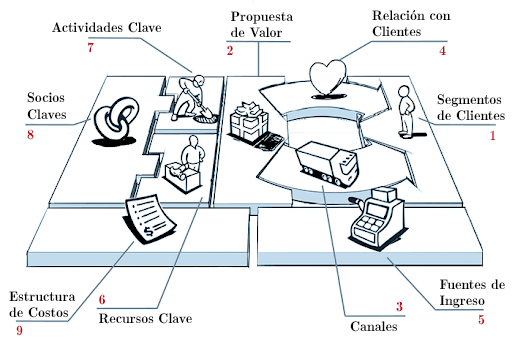
\includegraphics[width=0.75\textwidth]{./Figuras/diagCanvas.png}
\caption{Diagrama del nodelo canvas del negocio}
\label{fig:diagCanvas}
\end{figure}

\begin{enumerate}
\item Segmentos de cliente:
\begin{itemize}
\item Oficinas, centros educativos, hoteles, centros de salud, edificios de departamentos y centros comerciales.  
\item Grupos familiares en general.
\end{itemize}
\item Propuesta de valor:
\begin{itemize}
\item Consumo energético detallado por componente eléctrico/electrodoméstico.
\item Control y gestión de confort de distintos ambientes.
\end{itemize}
\item Canales:
   \begin{itemize}
\item Pagina web del producto.
\item Centros comerciales de tecnología.
\item Tiendas de domótica.
\item Empresas que ofrecen soluciones de automatización para hogares, oficinas, etc.
\end{itemize}
\item Relación con clientes:
\begin{itemize}
\item Centro de información y soporte técnico mediante web.
\item Central telefónica para atender emergencias relacionas al uso del sistema IOT.
\item Una App para dispositivos móviles para solicitar asesoría de uso de los productos o la visita de un técnico. 
\end{itemize}
\item Fuentes de ingreso:
\begin{itemize}
\item Venta del módulo principal y módulos de sensores básicos.
\item Venta del sistema IOT completo.
\item Venta de módulos de sensado de energía individual con su respectiva App.
\item Pago por servicio técnico.
\item Pago por consumo de nuestro servicio en la nube.
\end{itemize}
\item Recursos clave:
\begin{itemize}
\item Diseño pequeño, tecnológico y elegante del módulo del sistema principal para usar en casa u otro ambiente.
\item Bajo consumo energético del módulo principal y módulos.
\item Interfaz de usuario amigable y de fácil uso.
\item Sistema seguro y de fácil instalación.
\item Sistema en nube para controlar los Brokers remotos de los clientes.
\item Equipo de investigación y desarrollo.
\item Componentes electrónicos y partes necesarias para la fabricación de módulos.
\end{itemize}
\item Actividades clave:
\begin{itemize}
\item Estrategias de marketing.
\item Investigación y desarrollo.
\item Diseños de presentación de los módulos del sistema.
\item Producción y pruebas de productos.
\item Seguimiento del funcionamiento de los sistemas instalados a clientes.
\item Atención rápida a solicitudes de soporte técnico y asesoría de los productos. 
\end{itemize}
\item Socios claves:
\begin{itemize}
\item Proveedores de componentes electrónicos y partes necesarias para la fabricación de módulos.
\item Empresas que ofrecen servicios de almacenamiento y gestión de recursos en nube.
\item Tiendas de tecnología y automatización.
\item Centros comerciales de tecnología.
\item Empresas dedicadas a la instalación de soluciones domóticas.
\item Organizadores de eventos y exposiciones de productos tecnológicos.
\end{itemize}
\item Estructura de costos:
\begin{itemize}
\item Costos del equipo de I+D.
\item Costos de fabricación y producción.
\item Costos de almacenamiento y servicios en la nube.
\item Costos por estrategias y ejecución de marketing.
\item Costos por el equipo de atención al cliente.
\item Costos por actividades de desarrollo de negocios (alianzas y convenios).
\end{itemize}
\end{enumerate}

\section{Identificación y análisis de los interesados}
\label{sec:interesados}

En la siguiente tabla se muestra de  forma resumida los stakeholders del presente proyecto.
\begin{table}[ht]
%\caption{Identificación de los interesados}
%\label{tab:interesados}
\begin{tabularx}{\linewidth}{@{}|l|X|X|l|@{}}
\hline
\rowcolor[HTML]{C0C0C0} 
Rol           & Nombre y Apellido & Organización 	& Puesto 	\\ \hline
Cliente       & \clientename      &\empclientename	&   Administrativo  	\\ \hline
Responsable   & \authorname       & FIUBA        	& Alumno 	\\ \hline
Colaborador &  Leoncio Moya Carranza &      ICF Network 	&      Ing. redes y servidores 	\\ \hline
Orientador    & \supname	      & \pertesupname 	& Director	trabajo final \\ \hline
Usuario final & Grupos familiares en general.\newline    
				Empresas del sector hotelero, salud y cualquier sector comercial. &    -        & Propietario/Jefe \\ \hline


\end{tabularx}
\end{table}

Principales características de cada interesado.

\begin{itemize}
\item Cliente: Gabriela de la Cruz, es rigurosa y observadora en los detalles.
\item Responsable: Daniel Iván Cruz Flores, también es el único personal del equipo de desarrollo.
\item Colaboradores: Leoncio Moya Carranza ayuda mucho en el diseño y la configuración de redes.
\item Orientador: \supname, va a poder ayudar mucho con la gestión y formulación del proyecto.
\item Usuario Final: Hogares o empresas que desean tener información detalla para gestionar el consumo energético y contar con algunas características de confort.
\end{itemize}

\section{1. Propósito del proyecto}
\label{sec:proposito}

%\begin{consigna}{red}
El proposito de este proyecto es diseñar y desarrollar un sistema informático capaz de controlar y monitorear viviendas u otros ambientes mediante el protocolo MQTT para brindar una gestión inteligente respecto a confort y consumo energético.

%\end{consigna}

\section{2. Alcance del proyecto}
\label{sec:alcance}

El proyecto incluye: 
\begin{itemize}
\item Diseño y desarrollo del módulo principal.
\item Diseño y desarrollo del módulo réplica.
\item Diseño y desarrollo del módulo consumo.
\item Diseño y desarrollo del módulo temperatura.
\item Diseño y desarrollo del módulo actuador.
\end{itemize}

El presente proyecto no incluye el desarrollo del ``módulo inteligente'' y futuros módulos de interacción por voz Humano - Computador. Dichos módulos serán temas de desarrollo en trabajos futuros.

\section{3. Supuestos del proyecto}
\label{sec:supuestos}

Para el desarrollo del presente proyecto se supone que: 
\begin{itemize}
\item El cliente cuenta con una red LAN y con conexión a Internet.
\item El cliente cuenta con los componentes básicos de red para la creación de una red LAN dedicada.
\item El cliente cuenta con conocimientos mínimos de informática.
\item Se dispondrá del tiempo y recursos para desarrollar los módulos de hardware.
\item Los tiempos para el desarrollo de la aplicación web principal estará dentro de los márgenes establecidos.
\end{itemize}

%Por ejemplo, se podrían incluir supuestos respecto a disponibilidad de tiempo y recursos humanos y materiales, sobre la factibilidad técnica de distintos aspectos del proyecto, sobre otras cuestiones que sean necesarias para el éxito del proyecto como condiciones macroeconómicas o reglamentarias.



\section{4. Requerimientos}
\label{sec:requerimientos}

Los requerimientos se enumeran agrupados por afinidad:

\begin{enumerate}
\item Grupo de requerimientos asociados al ``módulo principal''.
	\begin{enumerate}
	\item El módulo debe tener instalado un servidor web.
	\item El módulo debe tener instalado un gestor de base de datos MySql.
	\item El módulo debe tener instalado un Broker.
	\item El módulo debe tener instalado Pyhton 3.x.
	\item El módulo debe tener un programa ejecutándose en segundo plano para detectar los valores que llegan al Broker y enviarlo a la base de datos local.
	\item El módulo debe tener ejecutándose en segundo plano un programa que replicará hacia la nube los datos que reciba el Broker local mientras tenga acceso a Internet.
	\item El módulo al ser encendido debe iniciar automáticamente el servidor web, el gestor de base de datos, el Broker, el programa de captura de datos para el envío a la base de datos y el programa que hace la réplica a la nube.
	\item El módulo debe tener una aplicación web para mostrar de forma amigable los datos capturados para permitir la gestión, control y monitoreo del sistema IOT.
	\item La aplicación debe leer los datos que llegan al Broker y mostrarlo vía web para comprobar que existe comunicación constante con el resto de módulos del sistema.
	\item La aplicación debe reportar los datos que llegan la base de datos mediante AJAX (Asynchronous JavaScript and XML).
	\item La aplicación debe mostrar información resumida mediante gráficos estadísticos y tablas detalladas de los sensores y módulos del sistema.
	\item La aplicación debe permitir generar reportes detallados en PDF de los datos capturados en la base de datos.
	\item La aplicación debe mostrar reportes del consumo energético actual por sensor.
	\item La aplicación debe mostrar los estados de los sensores (conectado, encendido o apagado) en tiempo real.	
	\item La aplicación debe permitir el acceso de 2 tipos de usuarios: el administrador con permisos totales del sistema y el usuario que solo desea ver información.
	\item La aplicación web deberá seguir funcionando correctamente si existiera algún corte de acceso a Internet.
	\item La aplicación debe contar con un protector de pantalla para cuando no se este interactuando (prioridad menor).
	\end{enumerate}
%%%%%%%%%%%%%%%%%%%%%%%%%%%%%%%%%%%%%%%%%%%%%%%%%%%%%%%%%%%%%%%%%%%%%	
\item Grupo de requerimientos asociados al ``módulo réplica''.
	\begin{enumerate}
	\item El módulo debe tener una aplicación web para mostrar de forma amigable los datos replicados del sistema IOT.
	\item La aplicación web estará almacenada en un servicio de servidor web remoto (Hosting).
	\item La aplicación web debe leer todos los datos que llegan al Broker remoto de réplica.
	\item La aplicación web debe ser estructurada con la característica de adaptabilidad para su acceso desde dispositivos portátiles.
	\item La aplicación debe mostrar reportes del consumo energético actual por sensor.
	\item La aplicación debe mostrar los estados de los sensores (conectado, encendido o apagado) en tiempo real.	
	\item La aplicación deberá mostrar un mensaje de alerta cuando el sistema principal local perdió conexión y no puede enviar los valores en tiempo real.
	\item La aplicación debe permitir el acceso de 2 tipos de usuarios: el administrador con permisos totales del sistema y el usuario que solo desea ver información.
	\end{enumerate}
%%%%%%%%%%%%%%%%%%%%%%%%%%%%%%%%%%%%%%%%%%%%%%%%%%%%%%%%%%%%%%%%%%%%
\item Grupo de requerimientos asociados al ``módulo consumo''.
	\begin{enumerate}
	\item El módulo debe usar una conexión Micro-USB para su fuente de alimentación de la placa principal.
	\item El módulo debe leer cada 5 segundos los datos del sensor de corriente.
	\item El módulo debe tener configurado las credenciales necesarias para unirse a la red local mediante Wifi.
	\item El módulo debe enviar sus lecturas obtenidas mediante el protocolo MQTT hacia el Broker del módulo principal central.
	\item El módulo debe estar funcionando 24/7.
	\item El módulo debe tener un case para protección de sus componentes internos y para su mejor presentación (prioridad menor).
	\end{enumerate}	
%%%%%%%%%%%%%%%%%%%%%%%%%%%%%%%%%%%%%%%%%%%%%%%%%%%%%%%%%%%%%%%%%%%%%	
\item Grupo de requerimientos asociados al ``módulo temperatura''.
	\begin{enumerate}
	\item El módulo debe usar una conexión Micro-USB para su fuente de alimentación para la placa principal.
	\item El módulo debe leer cada 2 segundos los datos del sensor de temperatura.
	\item El módulo debe tener configurado las credenciales necesarias para unirse a la red local mediante Wifi.
	\item El módulo debe enviar sus lecturas obtenidas mediante el protocolo MQTT hacia el Broker del módulo principal central.
	\item El módulo debe estar funcionando 24/7.
	\item El módulo debe tener un case para protección de sus componentes internos y para su mejor presentación(prioridad menor)
	\end{enumerate}	
%%%%%%%%%%%%%%%%%%%%%%%%%%%%%%%%%%%%%%%%%%%%%%%%%%%%%%%%%%%%%%%%%%%%%
\item Grupo de requerimientos asociados al ``módulo actuador''.
	\begin{enumerate}
	\item El módulo debe usar una conexión Micro-USB para su fuente de alimentación para la placa principal.
		\item El módulo debe recibir datos mediante el protocolo MQTT desde el Broker del módulo principal central.
	\item El módulo debe leer cada 1 segundo los datos que se le envían desde el módulo principal.
	\item El módulo debe tener configurado las credenciales necesarias para unirse a la red local mediante Wifi.
	\item El módulo debe estar funcionando 24/7.
	\item El módulo deberá estar conectado a un ventilador y actuara mediante un relé para su encendido o apagado del mismo.
	\item El módulo debe tener un case para protección de sus componentes internos y para su mejor presentación(prioridad menor)
	\end{enumerate}

\item Grupo de requerimientos asociados a la ``red local''.
	\begin{enumerate}
	\item La red local debe estar configurada con direcciones IP estáticas.
	\item La red local debe estar configurada con un access point para garantizar la fácil conexión entre módulos del sistema IOT así como extender el rango de la señal wifi.
	\item El access point de la red debe estar configurado en un canal de comunicación que no tenga solapamiento de canales wifi.
	\item La conexión a la red del pc del usuario administrador y de la pantalla monitor debe estar conectado vía cable Ethernet(prioridad menor).
	\end{enumerate}

\end{enumerate}

\section{Historias de usuarios (\textit{Product backlog})}
\label{sec:backlog}
Como criterio de ponderación se utilizó la serie de Fibonacci.
\begin{itemize}
\item Como administrador del sistema quiero poder saber el estado de cada sensor para poder garantizar un correcto reporte de información en la aplicación.\newline
Ponderación: 13
\item Como administrador del sistema quiero poder saber cuántos sensores tengo conectados para poder conocer qué porcentaje del total están orientados al monitoreo de televisores.\newline Ponderación: 21
\item Como administrador del sistema quiero poder acceder de forma remota desde mi laptop al sistema réplica para verificar la comunicación constante entre el sistema central local y el remoto.\newline Ponderación: 34
\item Como cliente quiero consultar el consumo de energía por uso de ventiladores para poder conocer el costo de consumo por ventilador. \newline Ponderación: 21
\item Como cliente quiero consultar el consumo de energía por uso de lámparas para poder conocer el horario promedio de mayor demanda. \newline Ponderación: 21
\item Como cliente quiero saber cuál es el ambiente con máxima y mínima temperatura para poder estimar la instalación de ventiladores en lugares donde se requiera. \newline Ponderación: 34
\item Como cliente quiero poder acceder al sistema de forma remota desde mi Tablet para poder verificar si deje alguna luz o ventilador encendido al salir de casa. \newline Ponderación: 34
\item Como cliente quiero obtener reportes detallados de consumo energético de los días que se cortó la conexión a Internet para verificar el funcionamiento del sistema y comparar el consumo con otro día cualquiera. \newline Ponderación: 55
\end{itemize}

\section{5. Entregables principales del proyecto}
\label{sec:entregables}
\begin{itemize}
\item Manual de uso.
\item Diagrama esquemático.
\item Diagrama de los componentes que forman el sistema.
\item Vídeo demostrativo de las pruebas de funcionamiento.
\item Informe final.
\end{itemize}
\section{6. Desglose del trabajo en tareas}
\label{sec:wbs}
Las tareas se muestran agrupados para una mejor comprensión:
%%%%%%%%%%%%%%%%%%%%%%%%%%%%%%%%%%%%%%%%%%%%%%%%%%%%%%%%%%%%%%%%%%%%%%%%%%
\begin{enumerate}
\item Búsqueda de material bibliográfico. (40 hs)
	\begin{enumerate}
	\item Búsqueda de soluciones similares en el mercado. (5 hs)
	\item Búsqueda de códigos fuente de ejemplos similares a los que se usará. (10 hs)
	\item Búsqueda de todos los componentes electrónicos a usar. (10 hs)
	\item Estudiar la forma de integración de componentes a la red. (10 hs)
	\item Estudiar cómo funciona cada uno de los componentes. (10 hs)
	\item Realizar un informe resumen con la lista de componentes, aspectos de red y configuraciones básicas a usar. (5 hs)
	\end{enumerate}
\item Adquisición de componentes. (20 hs)
	\begin{enumerate}
	\item Cotizar los costos de cada componente electrónico con los proveedores. (10 hs)
	\item Realizar los pedidos a proveedores. (5 hs)
	\item Realizar un informe de costos de los componentes adquiridos (5 hs)
	\end{enumerate}
%%%%%%%%%%%%%%%%%%%%%%%%%%%%%%%%%%%%%%%%%%%%%%%%%%%%%%%%%%%%%%%%%%%%%%%%%%%%%
\item Diseño y configuración de red local. (16 hs)
	\begin{enumerate}
	\item Instalación del modem/router en el lugar más adecuado. (2 hs)
	\item Instalación del access point en el lugar más adecuado. (2 hs)
	\item Configuración interna del modem/router y el access point. (2 hs)
	\item Verificación e instalación de los puntos de donde se conectarán los módulos sensores de muestreo. (5 hs)
	\item Realizar un informe de la configuración de red local instalada. (5 hs)
	\end{enumerate}
%%%%%%%%%%%%%%%%%%%%%%%%%%%%%%%%%%%%%%%%%%%%%%%%%%%%%%%%%%%%%%%%%%%%%%%%%%%%%
\item Desarrollo del módulo principal. (239 hs)
	\begin{enumerate}
	\item Instalación del sistema operativo en la Raspberry Pi (2 hs)
	\item Instalación y configuración del servidor web (5 hs)
	\item Instalación y configuración de Python 3 (2 hs)
	\item Instalación y configuración del Broker local (5 hs)
	\item Creación del programa para leer datos que llegan al Broker y enviarlo a la base de datos. (10 hs)
	\item Creación del programa para verificar constantemente el acceso a Internet (5 hs)
	\item Creación del programa para leer datos que llegan al Broker y replicarlos a la nube. (10 hs)
	\item Creación y configuración del script lanzador que iniciará automáticamente los programas al encender el módulo. (5 hs)
	\item Testeo del funcionamiento y conexión del módulo a la red local. (5 hs)
	\item Diseño y creación de la base de datos. (10 hs)
	\item Diseño y maquetación de la aplicación web principal. (40 hs)
	\item Desarrollo de todas las funcionalidades backend de la aplicación. (40 hs)
	\item Integración de todas las funcionalidades backend con el frontend de la aplicación web (20 hs)
	\item Creación de los tipos de reportes que ofrecerá la aplicación. (40 hs)
	\item Testeo y depuración del funcionamiento de los roles de acceso al sistema. (10 hs)
	\item Testeo y depuración del funcionamiento de la aplicación web en el pc del administrador. (5 hs)
	\item Testeo y depuración del funcionamiento de la aplicación web en el monitor informativo. (10 hs)
	\item Testeo y depuración del funcionamiento del sistema del módulo principal en situaciones de corte del acceso a Internet. (10 hs) 
	\item Realizar un informe resumen de las características del módulo, aspectos de red, configuraciones a usar, credenciales de acceso del usuario root, versiones del software, credenciales de acceso a la administración a la base de datos y a la aplicación web. (5 hs)
	\end{enumerate}

%%%%%%%%%%%%%%%%%%%%%%%%%%%%%%%%%%%%%%%%%%%%%%%%%%%%%%%%%%%%%%%%%%%%%%%%%%%%%%%%%
\item Desarrollo del módulo de consumo. (55 hs)
	\begin{enumerate}
	\item Construcción del módulo e integración de componentes, sensor de corriente con placa NodeMCU Esp8266. (15 hs)
	\item Creación del programa para leer datos del sensor. (10 hs)
	\item Testeo de conexión del módulo a la red y al módulo principal central. (5 hs)
	\item Testeo y depuración del envío de datos al módulo principal en la red local. (5 hs)
	\item Verificación y formateo de datos capturados por el sensor para su envío al módulo central. (10 hs)
	\item Instalación del módulo en un ambiente determinado para su funcionamiento. (5 hs)
	\item Realizar un informe resumen de las configuraciones a usar, código fuente e información respecto al formato de envío de datos. (5 hs)
	\end{enumerate}
%%%%%%%%%%%%%%%%%%%%%%%%%%%%%%%%%%%%%%%%%%%%%%%%%%%%%%%%%%%%%%%%%%%%%%%%%%%%%%%%%%%
\item Desarrollo del módulo temperatura. (40 hs)
	\begin{enumerate}
	\item Construcción del módulo e integración de componentes, sensor de temperatura con placa NodeMCU Esp8266. (10 hs)
	\item Creación del programa para leer datos del sensor. (5 hs)
	\item Testeo de conexión del módulo a la red y al módulo principal central. (5 hs)
	\item Testeo y depuración del envío de datos al módulo principal en la red local. (5 hs)
	\item Verificación y formateo de datos capturados por el sensor para su envío al módulo central. (5 hs)
	\item Instalación del módulo en un ambiente determinado para su funcionamiento. (5 hs)
	\item Realizar un informe resumen de las configuraciones a usar, código fuente e información respecto al formato de envío de datos. (5 hs)
	\end{enumerate}
%%%%%%%%%%%%%%%%%%%%%%%%%%%%%%%%%%%%%%%%%%%%%%%%%%%%%%%%%%%%%%%%%%%%%%%%%%%%%%%%%%%%
\item Desarrollo del módulo actuador. (55 hs)
	\begin{enumerate}
	\item Construcción del módulo e integración de componentes, actuador con placa NodeMCU Esp8266. (15 hs)
	\item Creación del programa para leer datos que llegan de la red.(10 hs)
	\item Testeo de conexión del módulo a la red y al módulo principal central. (5 hs)
	\item Testeo y depuración de la recepción y envío de datos al módulo principal en la red local. (5 hs)
	\item Verificación y formateo de datos capturados de la red para su manipulación y transformación en ordenes de la placa hacia el relé.(10 hs)
	\item Instalación del módulo en un ambiente determinado para su funcionamiento. (5 hs)
	\item Realizar un informe resumen de las configuraciones a usar, código fuente e información respecto al formato de recepción de datos. (5 hs)
	\end{enumerate}
	
%%%%%%%%%%%%%%%%%%%%%%%%%%%%%%%%%%%%%%%%%%%%%%%%%%%%%%%%%%%%%%%%%%%%%%%%%%%%%%%%
\item Desarrollo del módulo réplica. (95 hs)
	\begin{enumerate}
	\item Creación y configuración del Broker remoto (5 hs)
	\item Integración del Broker remoto con el módulo principal local para las replicas(10 hs)
	\item Verificación y testeo de enlace del Broker local con el Broker remoto. (10 hs)
	\item Creación de la base de datos replica en la nube. (5 hs) 
	\item Adaptación de la copia de la aplicación web local para su funcionamiento en remoto. (25 hs)
	\item Configuración para la recepción de datos del Broker remoto hacia la aplicación en nube.  (10 hs)
	\item Testeo y depuración del funcionamiento de los roles de acceso al sistema. (5 hs) 
	\item Testeo y depuración del funcionamiento de la aplicación web desde el pc del administrador. (10 hs) 
	\item Testeo y depuración del funcionamiento de la aplicación en diferentes dispositivos portátiles. (10 hs)
	\item Realizar un informe resumen de las configuraciones a usar y credenciales de acceso a la cuenta de administración. (5 hs)
	\end{enumerate}	
%%%%%%%%%%%%%%%%%%%%%%%%%%%%%%%%%%%%%%%%%%%%%%%%%%%%%%%%%%%%%%%%%%%%%%%%%%%%%%%%%%%%%
\item Verificación y testeo del sistema completo. (50 hs)
	\begin{enumerate}
	\item Verificación y depuración del funcionamiento completo del sistema IOT en un ambiente de red local controlado (laboratorio) con acceso a Internet (5 hs)
	\item Verificación y depuración del funcionamiento de los roles de acceso del sistema IOT en un ambiente de red local controlado (laboratorio) con acceso a Internet (5 hs) 
	\item Verificación y depuración del funcionamiento completo del sistema IOT en un ambiente real con acceso a Internet vía red local(5 hs) 
	\item Verificación y depuración del funcionamiento completo del sistema IOT en un ambiente real sin acceso a Internet vía red local (10 hs) 
	\item Verificación y depuración del funcionamiento completo del sistema réplica IOT remoto desde un dispositivo portátil (10 hs)
	\item Verificación y depuración del funcionamiento completo del sistema réplica IOT remoto desde un dispositivo portátil cuando el módulo principal local se desconecta de Internet (10 hs)
	\item Realizar un informe resumen con las correcciones de las nuevas configuraciones a usar y todas las nuevas consideraciones de funcionamiento. (5 hs)
	\end{enumerate}
%%%%%%%%%%%%%%%%%%%%%%%%%%%%%%%%%%%%%%%%%%%%%%%%%%%%%%%%%%%%%%%%%%%%%%%%%%%%%%%%%%%%%	
%\item Propuestas y recomendaciones de mejora para la presentación del sistema IOT. (35 hs)
%	\begin{enumerate}
%	\item Creación de propuestas de mejora en el aspecto de presentación física para el módulo principal (5 hs)
%	\item Creación de propuestas de mejora en el aspecto de presentación física para cada uno de los módulos (5 hs)
%	\item Creación de propuestas de mejora para nuevas funcionalidades a considerar para su integración en trabajos futuros(5 hs)
	%	\item Creación del manual de usuario del sistema IOT. (10 hs)
%	\item Creación de un vídeo resumen explicativo comercial del funcionamiento del sistema (10 hs)
%	\end{enumerate}	
		
		
\end{enumerate}

Cantidad total de horas: (610 hs)

\section{7. Diagrama de Activity On Node}
\label{sec:AoN}

La unidad de tiempo del diagrama AoN que se muestra en la Figura \ref{fig:AoN}  esta expresada en horas.

\begin{table}[ht]
%\caption{Identificación de los interesados}
%\label{tab:interesados}
\begin{tabularx}{\linewidth}{@{}|l|X|X|l|@{}}
\hline
\rowcolor[HTML]{C0C0C0} 
Descripción        & Secuencia de Tareas    & Tiempo (horas) 	\\ \hline
Camino crítico 1   & 1 - 2 - 3 - 4 - 5 - 8 - 9 & 515	 \\ \hline
Camino no crítico  & 1 - 2 - 3 - 4 - 6 - 8 - 9 & 500	 \\ \hline
Camino crítico 2   & 1 - 2 - 3 - 4 - 7 - 8 - 9 & 515  \\ \hline
\end{tabularx}
\end{table}
Los caminos críticos se muestran con líneas en \textbf{negrita} de color azul y la secuencia de tareas de color celeste.
%La figura \ref{fig:AoN} fue elaborada con el paquete latex tikz y pueden consultar la siguiente referencia \textit{online}:

%\url{https://www.overleaf.com/learn/latex/LaTeX_Graphics_using_TikZ:_A_Tutorial_for_Beginners_(Part_3)\%E2\%80\%94Creating_Flowcharts}



\begin{figure}[htpb]
\centering 
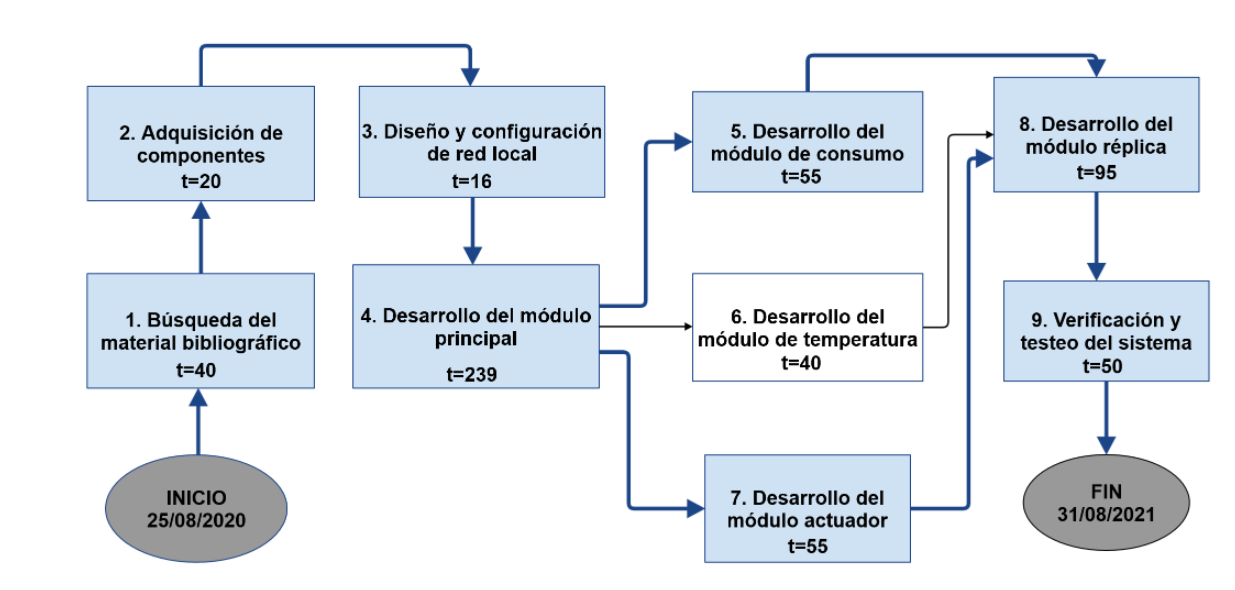
\includegraphics[width=1.0\textwidth]{./Figuras/AoN.png}
\caption{Diagrama en \textit{Activity on Node}}
\label{fig:AoN}
\end{figure}



\section{8. Diagrama de Gantt}
\label{sec:gantt}

%\begin{consigna}{red}
En las figuras \ref{fig:gantt1}, \ref{fig:gantt2}, \ref{fig:gantt3}, \ref{fig:gantt4}, se muestra a detalle el diagrama de Gantt del proyecto y en la figura \ref{fig:gantt5} se muestra un resumen del diagrama.
%%%%%%%%%%%%%%%%%%%%%%%%%%%%%%%%%%%%%%%%%
\begin{landscape} % esto es para rotar
\begin{figure}[htpb]
\centering 
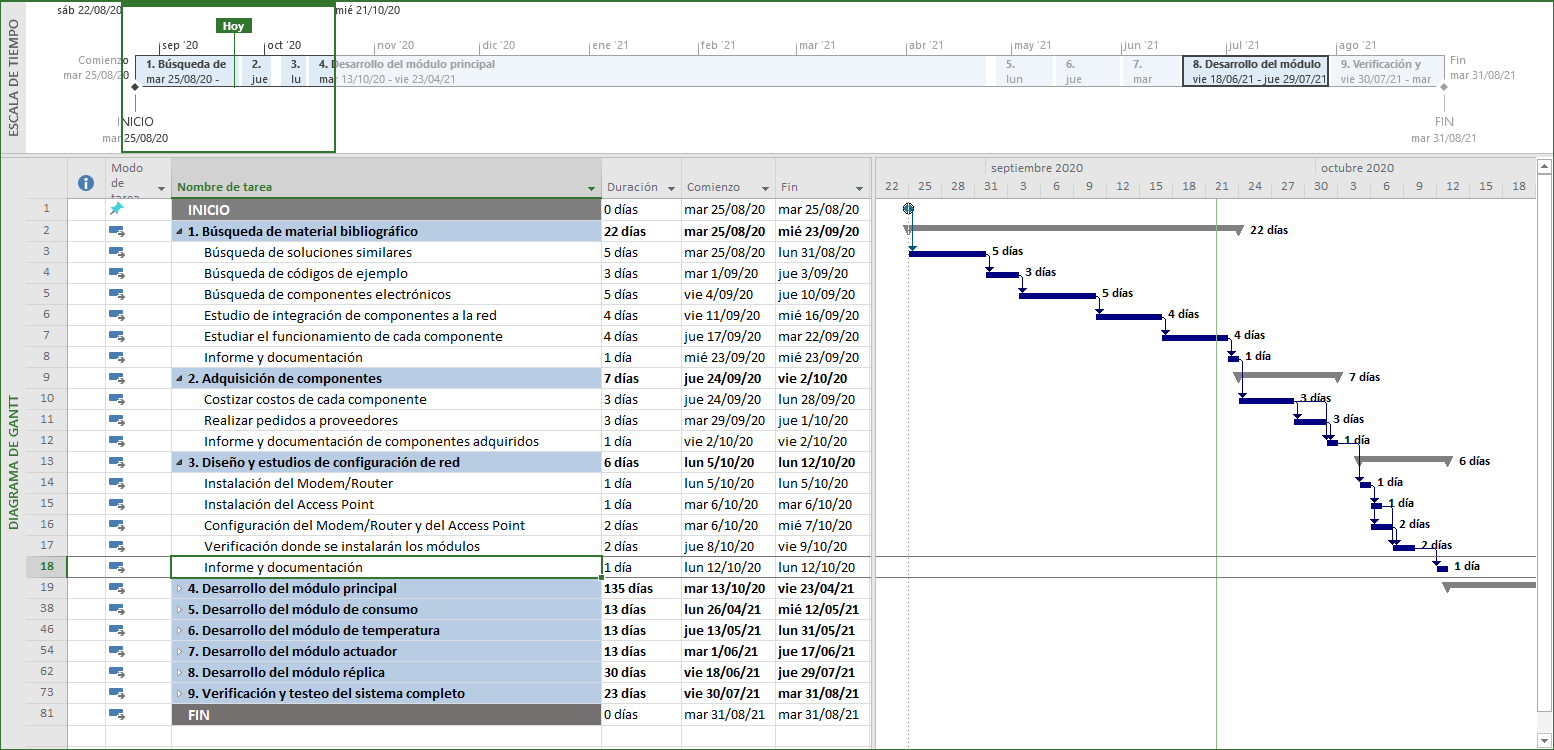
\includegraphics[width=1.5\textwidth]{./Figuras/gantt01.png}
\caption{Diagrama de Gantt - Parte 1}
\label{fig:gantt1}
\end{figure}
\end{landscape} % esto es para rotar
%%%%%%%%%%%%%%%%%%%%%%%%%%%%%%%%%%%%%%%%%%
\begin{landscape} % esto es para rotar
\begin{figure}[htpb]
\centering 
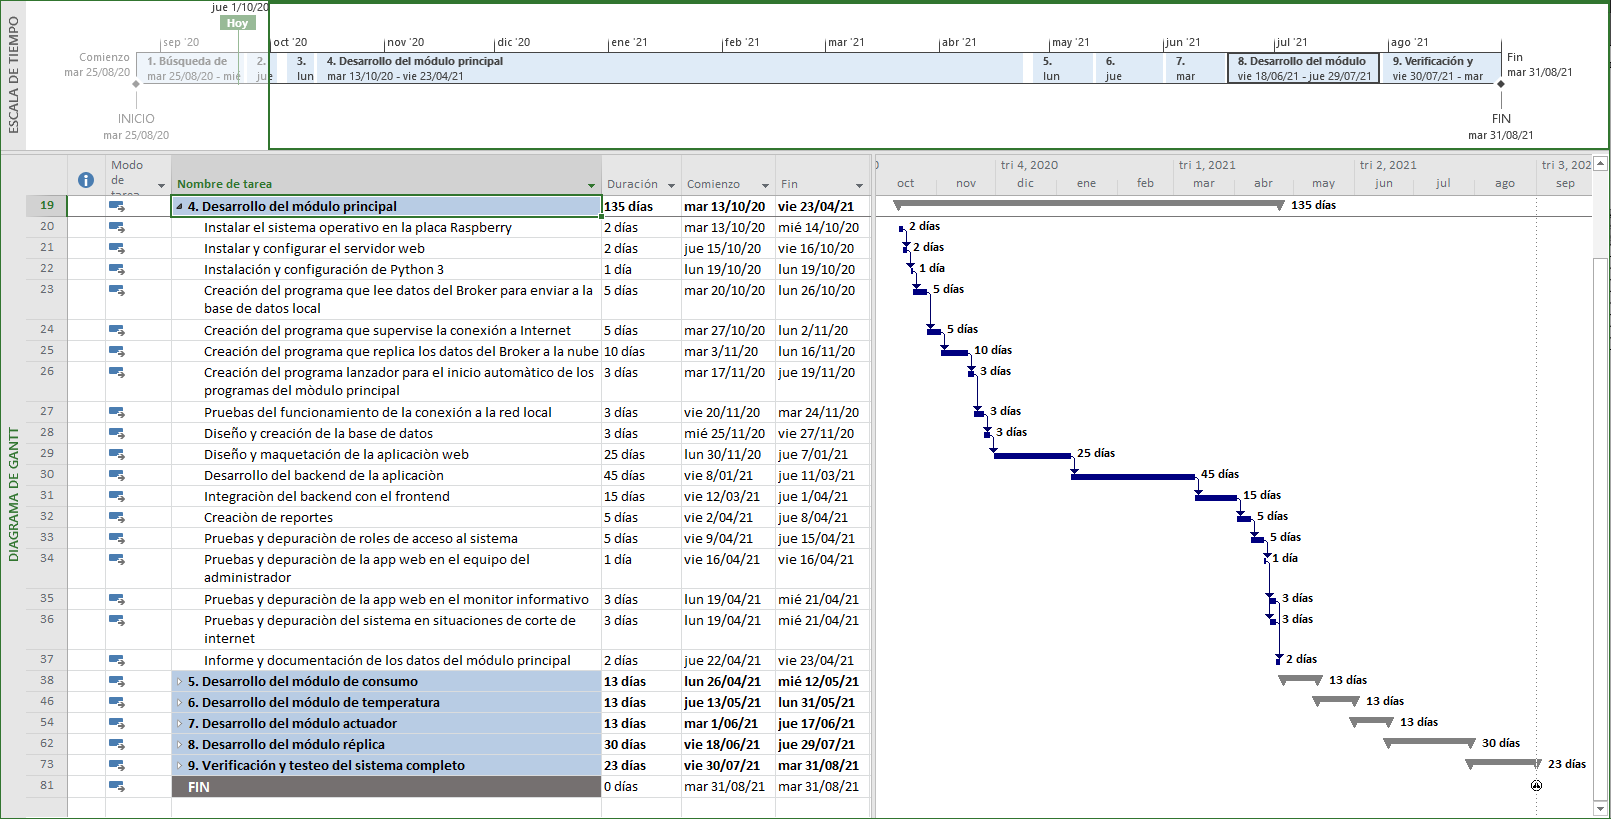
\includegraphics[width=1.5\textwidth]{./Figuras/gantt02.png}
\caption{Diagrama de Gantt - Parte 2}
\label{fig:gantt2}
\end{figure}
\end{landscape} % esto es para rotar
%%%%%%%%%%%%%%%%%%%%%%%%%%%%%%%%%%%%%%%%%%
\begin{landscape} % esto es para rotar
\begin{figure}[htpb]
\centering 
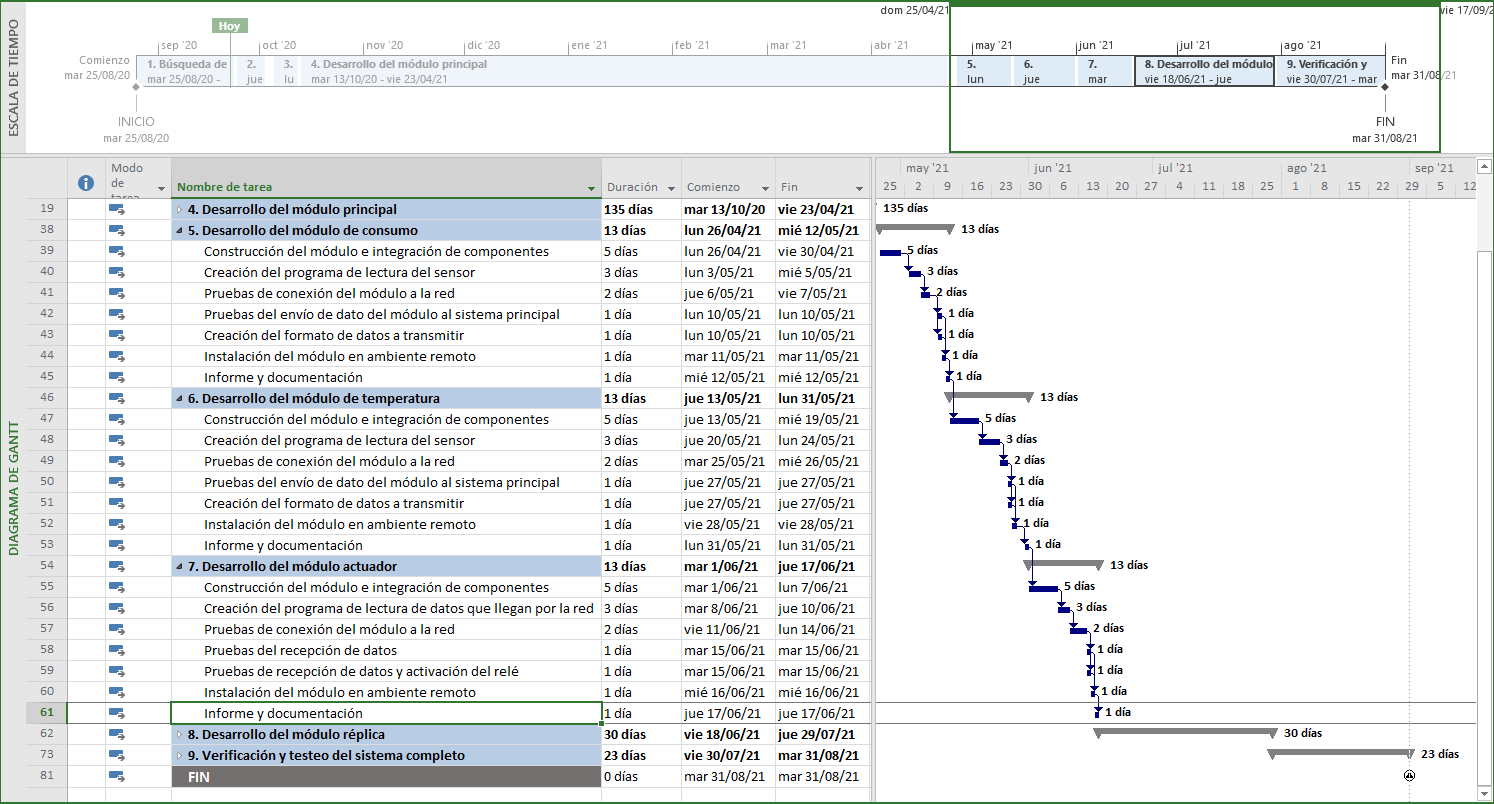
\includegraphics[width=1.5\textwidth]{./Figuras/gantt03.png}
\caption{Diagrama de Gantt - Parte 3}
\label{fig:gantt3}
\end{figure}
\end{landscape} % esto es para rotar
%%%%%%%%%%%%%%%%%%%%%%%%%%%%%%%%%%%%%%%%%%%%%
\begin{landscape} % esto es para rotar
\begin{figure}[htpb]
\centering 
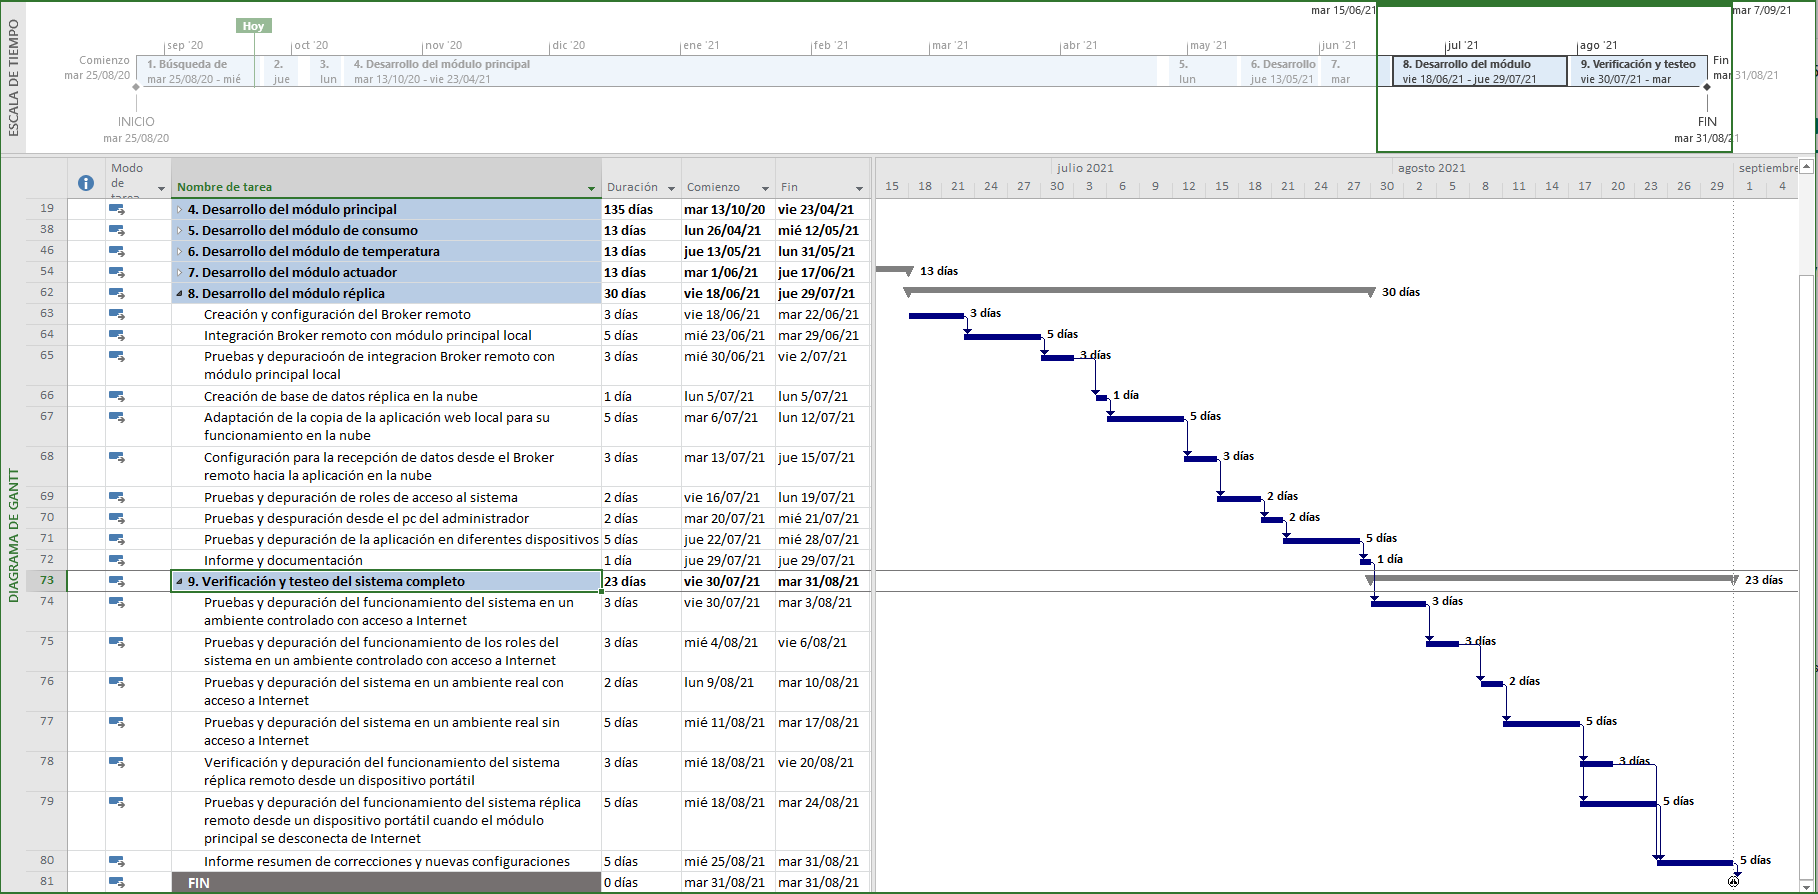
\includegraphics[width=1.5\textwidth]{./Figuras/gantt04.png}
\caption{Diagrama de Gantt - Parte 4}
\label{fig:gantt4}
\end{figure}
\end{landscape} % esto es para rotar
%%%%%%%%%%%%%%%%%%%%%%%%%%%%%%%%%%%%%%%%%%%

\begin{landscape} % esto es para rotar

\begin{figure}[htpb]
\centering 
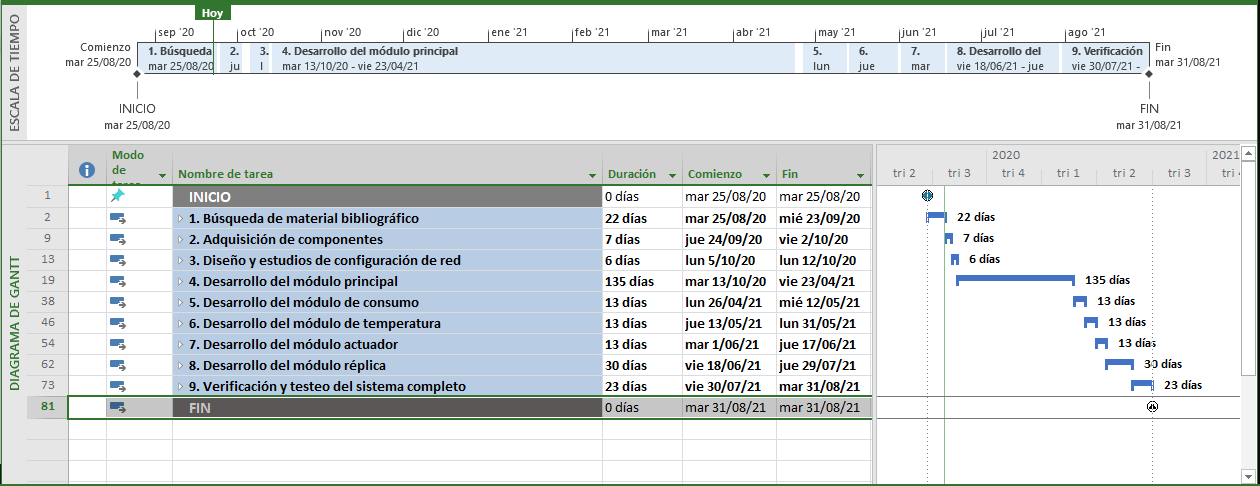
\includegraphics[width=1.5\textwidth]{./Figuras/gantt05.png}
\caption{Diagrama de Gantt resumido - Parte 5}
\label{fig:gantt5}
\end{figure}

\end{landscape} % esto es para rotar
%\end{consigna}


\section{9. Matriz de uso de recursos de materiales}
\label{sec:recursos}

\begin{table}[ht]
%\label{tab:recursos}
\centering
\begin{tabularx}{\linewidth}{@{}|c|X|c|c|c|c|@{}}
\hline
\cellcolor[HTML]{C0C0C0} & \cellcolor[HTML]{C0C0C0} & \multicolumn{4}{c|}{\cellcolor[HTML]{C0C0C0}Recursos requeridos (horas)} \\ \cline{3-6} 
\multirow{-2}{*}{\cellcolor[HTML]{C0C0C0}\begin{tabular}[c]{@{}c@{}}Código\\ WBS\end{tabular}} & \multirow{-2}{*}{\cellcolor[HTML]{C0C0C0}\begin{tabular}[c]{@{}c@{}}Nombre \\ tarea\end{tabular}} & Raspberry Pi & Sensores & Laptop & Internet \\ \hline
 1& Búsqueda de material bibliográfico & 0 & 0 & 20 & 20 \\ \hline
 2 & Adquisición de componentes & 0  & 0 & 10 & 10 \\ \hline
 3 & Diseño y configuración de la red local& 5 & 0 & 5 & 5 \\ \hline
 4 & Desarrollo del módulo principal & 239 & 0 & 200 & 200 \\ \hline
 5 & Desarrollo del módulo de consumo & 0 & 40 & 40 & 30 \\ \hline
 6 & Desarrollo del módulo de temperatura & 0 & 30 & 25 & 20 \\ \hline
 7 & Desarrollo del módulo actuador & 0 & 40 & 40 & 30 \\ \hline
 8 & Desarrollo del modulo réplica & 95 & 95 & 95 & 95 \\ \hline 
 9 & Pruebas y depuración del sistema completo & 50 & 50 & 50 & 40 \\ \hline
 %&  &  &  &  &  \\ \hline
\end{tabularx}%
\end{table}


\section{10. Presupuesto detallado del proyecto}
\label{sec:presupuesto}
%\begin{table}[htpb]
El presupuesto se muestra en moneda extranjera, ``Nuevo Sol'' de Perú (S/)
\begin{table}[ht]
\centering
\begin{tabularx}{\linewidth}{@{}|X|c|r|r|@{}}
\hline
\rowcolor[HTML]{C0C0C0} 
\multicolumn{4}{|c|}{\cellcolor[HTML]{C0C0C0}COSTOS DIRECTOS} \\ \hline
\rowcolor[HTML]{C0C0C0} 
\multicolumn{4}{|l|}{\cellcolor[HTML]{C0C0C0}MÓDULO CENTRAL - PRINCIPAL} \\ \hline
\rowcolor[HTML]{C0C0C0} 
Descripción &
  \multicolumn{1}{c|}{\cellcolor[HTML]{C0C0C0}Cantidad} &
  \multicolumn{1}{c|}{\cellcolor[HTML]{C0C0C0}Valor unitario} &
  \multicolumn{1}{c|}{\cellcolor[HTML]{C0C0C0}Valor total} \\ \hline
 Kit Raspberry Pi 4- 8GB & 
  \multicolumn{1}{c|}{1} &
  \multicolumn{1}{c|}{350} &
  \multicolumn{1}{c|}{350} \\ \hline
 Fuente de poder 5v 3A oficial Raspberry Pi 4B &
  \multicolumn{1}{c|}{1} &
  \multicolumn{1}{c|}{50} &
  \multicolumn{1}{c|}{50} \\ \hline
 Cable micro HDMI - HDMI &
  \multicolumn{1}{c|}{1} &
  \multicolumn{1}{c|}{30} &
  \multicolumn{1}{c|}{30} \\ \hline
  Micro SD Ultra - Clase 10 - 32 Gb &
  \multicolumn{1}{c|}{1} &
  \multicolumn{1}{c|}{35} &
  \multicolumn{1}{c|}{35} \\ \hline
  15.6 Touch Monitor, 1920×1080 Full HD &
  \multicolumn{1}{c|}{1} &
  \multicolumn{1}{c|}{680} &
  \multicolumn{1}{c|}{680} \\ \hline
  Case acrílico &
  \multicolumn{1}{c|}{1} &
  \multicolumn{1}{c|}{150} &
  \multicolumn{1}{c|}{150} \\ \hline
 
\multicolumn{3}{|r|}{SUBTOTAL} &
  \multicolumn{1}{c|}{S/ 1295} \\ \hline
%%%%%%%%%%%%%%%%%%%%%%%%%%%%%%%%%%%%%%%%%%%%%%%%%%%%%%%%%%%%
\rowcolor[HTML]{C0C0C0} 
\multicolumn{4}{|l|}{\cellcolor[HTML]{C0C0C0}MÓDULO DE CONSUMO ENERGÉTICO} \\ \hline
\rowcolor[HTML]{C0C0C0} 
Descripción &
  \multicolumn{1}{c|}{\cellcolor[HTML]{C0C0C0}Cantidad} &
  \multicolumn{1}{c|}{\cellcolor[HTML]{C0C0C0}Valor unitario} &
  \multicolumn{1}{c|}{\cellcolor[HTML]{C0C0C0}Valor total} \\ \hline
 Placa NodeMCU ESP8266 &
  \multicolumn{1}{c|}{1} &
  \multicolumn{1}{c|}{30} &
  \multicolumn{1}{c|}{30} \\ \hline
 Fuente de poder 5v – 1A &
  \multicolumn{1}{c|}{1} &
  \multicolumn{1}{c|}{15} &
  \multicolumn{1}{c|}{15} \\ \hline
  Case acrílico&
  \multicolumn{1}{c|}{1} &
  \multicolumn{1}{c|}{20} &
  \multicolumn{1}{c|}{20} \\ \hline
  Placa de circuito impreso &
  \multicolumn{1}{c|}{1} &
  \multicolumn{1}{c|}{10} &
  \multicolumn{1}{c|}{10} \\ \hline
  Sensor de corriente AC 30A no invasivo &
  \multicolumn{1}{c|}{1} &
  \multicolumn{1}{c|}{40} &
  \multicolumn{1}{c|}{40} \\ \hline
\multicolumn{3}{|r|}{SUBTOTAL} &
  \multicolumn{1}{c|}{S/ 115} \\ \hline
  \end{tabularx}%
\end{table}
  %%%%%%%%%%%%%%%%%%%%%%%%%%%%%%%%%%%%%%%
  
 \begin{table}
\centering
\begin{tabularx}{\linewidth}{@{}|X|c|r|r|@{}}
\hline 
\rowcolor[HTML]{C0C0C0} 
\multicolumn{4}{|c|}{\cellcolor[HTML]{C0C0C0}COSTOS DIRECTOS} \\ \hline
\rowcolor[HTML]{C0C0C0} 
\multicolumn{4}{|l|}{\cellcolor[HTML]{C0C0C0}MÓDULO DE MEDICIÓN DE TEMPERATURA} \\ \hline
\rowcolor[HTML]{C0C0C0} 
Descripción &
  \multicolumn{1}{c|}{\cellcolor[HTML]{C0C0C0}Cantidad} &
  \multicolumn{1}{c|}{\cellcolor[HTML]{C0C0C0}Valor unitario} &
  \multicolumn{1}{c|}{\cellcolor[HTML]{C0C0C0}Valor total} \\ \hline
  Placa NodeMCU ESP8266 &
  \multicolumn{1}{c|}{1} &
  \multicolumn{1}{c|}{30} &
  \multicolumn{1}{c|}{30} \\ \hline
  Fuente de poder 5v – 1A &
  \multicolumn{1}{c|}{1} &
  \multicolumn{1}{c|}{15} &
  \multicolumn{1}{c|}{15} \\ \hline
  Case acrílico &
  \multicolumn{1}{c|}{1} &
  \multicolumn{1}{c|}{20} &
  \multicolumn{1}{c|}{20} \\ \hline
  Placa de circuito impreso &
  \multicolumn{1}{c|}{1} &
  \multicolumn{1}{c|}{40} &
  \multicolumn{1}{c|}{40} \\ \hline
  Sensor de temperatura DHT 22 &
  \multicolumn{1}{c|}{1} &
  \multicolumn{1}{c|}{25} &
  \multicolumn{1}{c|}{25} \\ \hline
\multicolumn{3}{|r|}{SUBTOTAL} &
  \multicolumn{1}{c|}{S/ 100} \\ \hline
\rowcolor[HTML]{C0C0C0}

%%%%%%%%%%%%%%%%%%%%%%%%%%%%%%%%%%%%%%%%%%%%%%%%%%%%%%
\rowcolor[HTML]{C0C0C0} 
\multicolumn{4}{|l|}{\cellcolor[HTML]{C0C0C0}MÓDULO ACTUADOR} \\ \hline
\rowcolor[HTML]{C0C0C0} 
Descripción &
  \multicolumn{1}{c|}{\cellcolor[HTML]{C0C0C0}Cantidad} &
  \multicolumn{1}{c|}{\cellcolor[HTML]{C0C0C0}Valor unitario} &
  \multicolumn{1}{c|}{\cellcolor[HTML]{C0C0C0}Valor total} \\ \hline
 Placa NodeMCU ESP8266 &
  \multicolumn{1}{c|}{1} &
  \multicolumn{1}{c|}{30} &
  \multicolumn{1}{c|}{25} \\ \hline
  Fuente de poder 5v – 1A &
  \multicolumn{1}{c|}{1} &
  \multicolumn{1}{c|}{15} &
  \multicolumn{1}{c|}{15} \\ \hline
  Case acrílico &
  \multicolumn{1}{c|}{1} &
  \multicolumn{1}{c|}{20} &
  \multicolumn{1}{c|}{20} \\ \hline
  Placa de circuito impreso &
  \multicolumn{1}{c|}{1} &
  \multicolumn{1}{c|}{10} &
  \multicolumn{1}{c|}{10} \\ \hline
  Módulo Relay 1CH 5V DC &
  \multicolumn{1}{c|}{1} &
  \multicolumn{1}{c|}{10} &
  \multicolumn{1}{c|}{10} \\ \hline
  
\multicolumn{3}{|r|}{SUBTOTAL} &
  \multicolumn{1}{c|}{S/ 85} \\ \hline
  
  %%%%%%%%%%%%%%%%%%%%%%%%%%%%%%%%%%%%%%%%%%%%%%%%%%%%%%%%%%%%%%
 \rowcolor[HTML]{C0C0C0} 
\multicolumn{4}{|l|}{\cellcolor[HTML]{C0C0C0}OTROS GASTOS} \\ \hline
\rowcolor[HTML]{C0C0C0} 
Descripción &
  \multicolumn{1}{c|}{\cellcolor[HTML]{C0C0C0}Cantidad} &
  \multicolumn{1}{c|}{\cellcolor[HTML]{C0C0C0}Valor unitario} &
  \multicolumn{1}{c|}{\cellcolor[HTML]{C0C0C0}Valor total} \\ \hline
 AP 450mbps &
  \multicolumn{1}{c|}{1} &
  \multicolumn{1}{c|}{150} &
  \multicolumn{1}{c|}{150} \\ \hline
  Compra de un plan de hosting + dominio &
  \multicolumn{1}{c|}{1} &
  \multicolumn{1}{c|}{250} &
  \multicolumn{1}{c|}{250} \\ \hline
  Cable dupont macho- macho &
  \multicolumn{1}{c|}{4 paquetes} &
  \multicolumn{1}{c|}{60} &
  \multicolumn{1}{c|}{60} \\ \hline
  
\multicolumn{3}{|r|}{SUBTOTAL} &
  \multicolumn{1}{c|}{S/ 460} \\ \hline
\rowcolor[HTML]{C0C0C0}
\multicolumn{3}{|r|}{TOTAL} &
 \multicolumn{1}{c|}{S/ 2055}  \\ \hline   

  \rowcolor[HTML]{C0C0C0} 
\multicolumn{4}{|c|}{\cellcolor[HTML]{C0C0C0}COSTOS INDIRECTOS} \\ \hline
\rowcolor[HTML]{C0C0C0} 
Descripción &
  \multicolumn{1}{c|}{\cellcolor[HTML]{C0C0C0}Cantidad} &
  \multicolumn{1}{c|}{\cellcolor[HTML]{C0C0C0}Valor unitario} &
  \multicolumn{1}{c|}{\cellcolor[HTML]{C0C0C0}Valor total} \\ \hline
45\% respecto a costos directos  &
  \multicolumn{1}{c|}{1} &
  \multicolumn{1}{c|}{924.75} &
  \multicolumn{1}{c|}{924.75} \\ \hline

\multicolumn{3}{|r|}{SUBTOTAL} &
  \multicolumn{1}{c|}{S/ 924.75} \\ \hline
\rowcolor[HTML]{C0C0C0}
\multicolumn{3}{|r|}{TOTAL} &
\multicolumn{1}{c|}{S/ 2979.75}   \\ \hline
\end{tabularx}%
\end{table}


\begin{landscape} % esto es para rotar
\section{11. Matriz de asignación de responsabilidades}
\label{sec:responsabilidades}
%\begin{consigna}{red}


\begin{table}[htpb]
%\begin{center}
%\begin{sideways} % rotamos 90° la tabla
\centering
\resizebox{1.4\textwidth}{!}{%
\begin{tabular}{|c|l|c|c|c|c|}
\hline
\rowcolor[HTML]{C0C0C0} 
\cellcolor[HTML]{C0C0C0} &
  \cellcolor[HTML]{C0C0C0} &
  \multicolumn{4}{c|}{\cellcolor[HTML]{C0C0C0}Listar todos los nombres y roles del proyecto} \\ \cline{3-6} 
\rowcolor[HTML]{C0C0C0} 
\cellcolor[HTML]{C0C0C0} &
  \cellcolor[HTML]{C0C0C0} &
  Responsable &
  Orientador &
  Equipo &
  Cliente \\ \cline{3-6} 
\rowcolor[HTML]{C0C0C0} 
\multirow{-3}{*}{\cellcolor[HTML]{C0C0C0}\begin{tabular}[c]{@{}c@{}}Código\\ WBS\end{tabular}} &
  \multirow{-3}{*}{\cellcolor[HTML]{C0C0C0}Nombre de la tarea} &
  \authorname &
  \supname &
  Leoncio Moya &
  \clientename \\ \hline
 1& Búsqueda de material bibliográfico & P & C &  &  \\ \hline
 2& Adquisición de componentes & P & C & C &  \\ \hline
 3&Diseño y configuración de red local & P  & A & S &  \\ \hline
 4&Desarrollo del módulo principal & P & A & C & I \\ \hline
 5& Desarrollo del módulo de consumo & P  & A &  & C \\ \hline
 6& Desarrollo del módulo temperatura & P & A &  & C \\ \hline
  7& Desarrollo del módulo actuador & P  & A &  & C \\ \hline
 8& Desarrollo del módulo réplica & P & A & C & I \\ \hline
 9& Verificación y testeo del sistema completo & P & A & C & A \\ \hline
\end{tabular}%
}
%\end{sideways}% para rotación
%\end{center}
\end{table}

{\footnotesize
Referencias:

\begin{itemize}

	 \item P = Responsabilidad Primaria
	 \item S = Responsabilidad Secundaria
	 \item A = Aprobación
	 \item I = Informado
	 \item C = Consultado
\end{itemize}
} %footnotesize

\end{landscape}

%\end{consigna}


\section{12. Gestión de riesgos}
\label{sec:riesgos}

a) Identificación de los riesgos. 

Los riesgos listados a continuación será cuantificados en un rango del 1 al 10:
\begin{itemize}
\item Severidad (S): cuánto más severo el riesgo, más alto el número. 
\item Ocurrencia (O): cuánto más probable es que ocurra el riesgo, más alto el número.
\end{itemize}

Riesgo 1: no cumplir con los requerimientos pactados con el cliente.
\begin{itemize}
\item Severidad (9): el producto no funciona o no tiene la funcionalidad mínima esperada para el sistema.
\item Probabilidad de ocurrencia (4): porque se considera dedicar tiempo semanal para la creación de la aplicación y fabricación de componentes del sistema. 
\end{itemize}   

Riesgo 2: no contar a tiempo con las placas y sensores a utilizar.
\begin{itemize}
\item Severidad (10): conlleva a la no implementación del sistema. 
\item Ocurrencia (4): porque cada componente electrónico a usar se pedirá con anticipación considerando que de ellos depende la fabricación de componentes que integran el sistema.
\end{itemize}

Riesgo 3: errores de diseño, fabricación e integración de componentes electrónicos en el PCB de los módulos del prototipo.
\begin{itemize}
\item Severidad (5): conlleva al mal funcionamiento de los sensores.
\item Ocurrencia (3): porque se tiene un estudio previo, un diseño y una verificación mediante simulación para garantizar su correcta integración y funcionamiento.

\end{itemize}

Riesgo 4: errores de transmisión y conexión de sensores por mala configuración inalámbrica de red local.
\begin{itemize}
\item Severidad (8): conlleva al no funcionamiento del sistema por pérdida de conexión con los módulos del sensores y actuadores.
\item Ocurrencia (3): porque se tiene un estudio previo, un diseño y apoyo de un colaborador del área de redes para garantizar la correcta construcción de la red dedicada.
\end{itemize}

Riesgo 5: no informar en la aplicación de la nube de la pérdida de conexión entre el módulo réplica y el módulo central local.
\begin{itemize}
\item Severidad (5): ocasiona confusión y mala información al usuario remoto.
\item Ocurrencia (3): porque se considera una de las funciones principales de la aplicación que estará en la nube y será desarrollado por un equipo que tiene experiencia en el tema.
\end{itemize}

Riesgo 6: falla o avería de la tarjeta MicroSD del módulo principal.
\begin{itemize}
\item Severidad (10): ocasiona la pérdida de la aplicación, de la base de datos local y que el sistema deje de funcionar.
\item Ocurrencia (3): porque somos muy cuidadosos con el prototipo.
\end{itemize}



b) Tabla de gestión de riesgos:      (El RPN se calcula como RPN=SxO)

\begin{table}[htpb]
\centering
\begin{tabularx}{\linewidth}{@{}|X|X|X|X|X|X|X|@{}}
\hline
\rowcolor[HTML]{C0C0C0} 
Riesgo & S & O & RPN & S* & O* & RPN* \\ \hline
  1     & 9  & 4  & \cellcolor[HTML]{f5b7b1} 36    & 5   &  2  &   \cellcolor[HTML]{d6eaf8} 10   \\ \hline
  2     &  10 & 4  & \cellcolor[HTML]{f5b7b1} 40   &  10  &  2  & \cellcolor[HTML]{d6eaf8} 20    \\ \hline
  3     &  5 & 3  & \cellcolor[HTML]{d6eaf8}  15  &    &    &      \\ \hline
  4     & 8  &  3 &\cellcolor[HTML]{d6eaf8}  24   &    &    &      \\ \hline
  5     & 5  &  3 & \cellcolor[HTML]{d6eaf8} 15   &    &    &      \\ \hline
  6     & 10  & 3  & \cellcolor[HTML]{f5b7b1} 30   & 5   & 2   & \cellcolor[HTML]{d6eaf8} 10    \\ \hline
\end{tabularx}%
\end{table}

Criterio adoptado: 
Se tomarán medidas de mitigación en los riesgos cuyos números de RPN sean mayores a 25

Nota: los valores marcados con (*) en la tabla corresponden luego de haber aplicado la mitigación.

c) Plan de mitigación de los riesgos que originalmente excedían el RPN máximo establecido:
 
 
Riesgo 1: no cumplir con los requerimientos pactados con el cliente.
\begin{itemize}
\item Plan de mitigación: se desarrollará un plan de control y seguimiento semanal para garantizar el cumplimiento de cada requerimiento funcional.
\item Severidad (5): un control estricto de seguimiento del proyecto permitirá desarrollar cada requerimiento en los plazos establecidos.
\item Probabilidad de ocurrencia (2): es muy poco probable no desarrollar un requerimiento realizando un seguimiento al desarrollo del proyecto. 
\end{itemize}  
 
Riesgo 2: no contar a tiempo con las placas y sensores a utilizar.
\begin{itemize}
\item Plan de mitigación: crear una lista de todos los proveedores de componentes electrónicos para tener opción a pedir en más de un proveedor cada uno de los elementos a usar en el proyecto.
\item Severidad (10): se mantiene porque en el peor de los casos siempre estará presente el riesgo de no tener componentes disponibles a tiempo. 
\item Ocurrencia (2): porque cada componente electrónico podemos pedirlo a más de un proveedor, y de esta manera ampliar las opciones de disponibilidad.
\end{itemize}

Riesgo 6: falla o avería de la tarjeta MicroSD del módulo principal.
\begin{itemize}
\item Plan de mitigación: tener 2 tarjetas MicroSD con copias iguales para ser usadas en el Raspberry Pi, se usará una dejando la otra en un lugar seguro.
\item Severidad (5): si falla una MicroSD hay otra de respaldo.
\item Ocurrencia (2): es muy baja la probabilidad de perder ambas copias.
\end{itemize}




\section{13. Gestión de la calidad}
\label{sec:calidad}

\begin{enumerate}
\item El sistema deberá tener un módulo principal central local para el monitoreo y control.

\begin{itemize}
\item Verificación: se comprobará que el módulo principal este implementado en una Raspberry Pi 4 con una aplicación web ejecutándose en su servidor web. La aplicación deberá mostrar gráficos estadísticos para una vista resumen y tablas para vistas detalladas. 
\item Validación: se harán pruebas de conexión entre el módulo central y los sensores inalámbricos para validar que los datos mostrados en la aplicación son los correctos en cualquier instante de tiempo. 
\end{itemize}

\item El sistema deberá tener un módulo réplica en la nube para el acceso remoto al sistema.

\begin{itemize}
\item Verificación: se comprobará que el módulo réplica ubicado en la nube tenga conexión con el módulo central local para permitir el acceso remoto al sistema, solo cuando el módulo central local tenga conexión a Internet.
\item Validación: se harán pruebas de envío de datos de forma remota desde el módulo réplica hacia el sistema central local para validar el enlace correcto entre módulos.  
\end{itemize}

\item El sistema contará con el desarrollo de un módulo de consumo energético para electrodomésticos.

\begin{itemize}
\item Verificación: se comprobará que la fabricación del módulo tenga integrado el sensor de corriente y la placa de NodeMCU Esp8266, así como su correcta conexión a la red inalámbrica.
\item Validación: se harán pruebas de envío de datos hacia el módulo principal y dichos valores deben ser mostrados en unidades de consumo energético y almacenados en la base de datos del módulo central local.
\end{itemize}

\item El sistema contará con el desarrollo de un módulo de temperatura para medir la temperatura de ambiente.

\begin{itemize}
\item Verificación: se comprobará que la fabricación del módulo tenga integrado el sensor de temperatura y la placa de NodeMCU Esp8266, así como su correcta conexión a la red inalámbrica. 
\item Validación: se harán pruebas de envío de datos hacia el módulo principal y dichos valores deben ser mostrados en grados Celsius con un tiempo de lectura periódica de 2 segundos y almacenados en la base de datos del módulo central local.  
\end{itemize}


\item El sistema contará con el desarrollo de un módulo actuador para el encendido y apagado de ventiladores.

\begin{itemize}
\item Verificación: se comprobará que la fabricación del módulo tenga integrado el relé actuador y la placa de NodeMCU Esp8266, así como su correcta conexión a la red inalámbrica.
\item Validación: se harán pruebas de lectura de datos que llegan por vía inalámbrica de forma periódica cada 1 segundo y el tiempo de respuesta de activación del relé debe ser menor o igual a 2 segundos.  
\end{itemize}

\item El sistema central y sensores deberán estar configurados en una red local.

\begin{itemize}
\item Verificación: se comprobará que la red creada para el funcionamiento local del sistema cuenta con la instalación y configuración correcta de componentes de red y que no interfiere con la red LAN de la vivienda o edificio. 
\item Validación: se harán pruebas de conexión inalámbrica de la señal y canal del funcionamiento del AP así como cobertura de señal en cada sector donde se encuentra un sensor o actuador del sistema. 
\end{itemize}

\end{enumerate}

\section{14. Comunicación del proyecto}
\label{sec:comunicaciones}

El plan de comunicación del proyecto es el siguiente:

\begin{table}[htpb]
\centering
\begin{tabularx}{\linewidth}{@{}|X|C{2.7cm}|C{2.3cm}|C{1.8cm}|C{2cm}|C{2.1cm}|@{}}
\hline
\rowcolor[HTML]{C0C0C0} 
\multicolumn{6}{|c|}{\cellcolor[HTML]{C0C0C0}PLAN DE COMUNICACIÓN DEL PROYECTO}           \\ \hline
\rowcolor[HTML]{C0C0C0} 
¿Qué comunicar? & Audiencia & Propósito & Frecuencia & Método de comunicac. & Responsable \\ \hline
    Plan del proyecto              &   Mg. Ing. Matías Alvarez       &          Planificación de tiempos, evitar errores &   Cada semana        &     email, videoconferencia                  &    Iván Cruz  Flores    \\ \hline
   Avance en el desarrollo de requerimientos             &  Mg. Ing. Matías Alvarez, Gabriela de la Cruz         &    Comunicar avance       &     Cada 2 semanas       &                     email, videoconferencia &     Iván Cruz  Flores        \\ \hline
   Consultas técnicas para el desarrollo de los módulos             &          Mg. Ing. Matías Alvarez, Leoncio Moya Carranza &     Sugerencias, evitar errores      &     Cada 2 semanas       &                      email, videoconferencia &     Iván Cruz  Flores        \\ \hline
  Etapa de pruebas y verificación              &   Mg. Ing. Matías Alvarez, Gabriela de la Cruz        &    Retroalimentación por parte del cliente       &    Cada mes        &                     email, videoconferencia &       Iván Cruz  Flores      \\ \hline
  Finalización del proyecto              &   Mg. Ing. Matías Alvarez, Gabriela de la Cruz        &   Presentación final del proyecto        &    Única vez al finalizar        &                     email, videoconferencia &      Iván Cruz  Flores       \\ \hline
\end{tabularx}
\end{table}

\section{15. Gestión de compras}
\label{sec:compras}
El proyecto requiere de la adquisición de una placa Raspberry Pi 4, placas NodeMCU ESP8266, sensores de corriente no invasivos y componentes electrónicos básicos que pueden ser adquiridos en cualquier comercio de componentes electrónicos de las ciudades de Perú, por lo que la definición de un proveedor queda sujeta a los distintos precios de venta y disponibilidad. El costo de cada componente electrónico y el servicio de almacenamiento en la nube/hosting será cubierto por el responsable del proyecto.


\section{16. Seguimiento y control}
\label{sec:seguimiento}

\begin{longtable}{|m{1cm}|m{3.5cm}|m{2.2cm}|m{2cm}|m{3cm}|m{1.5cm}|}
\hline
\rowcolor[HTML]{C0C0C0} 
\multicolumn{6}{|c|}{\cellcolor[HTML]{C0C0C0}SEGUIMIENTO DE AVANCE}                                                                       \\ \hline
\rowcolor[HTML]{C0C0C0} 
Tarea del WBS 			& Indicador de avance & Frecuencia de reporte & Resp. de seguimiento & Persona a ser informada & Método de comunic. \\ \hline
\endfirsthead

\hline
\rowcolor[HTML]{C0C0C0} 
\multicolumn{6}{c}{\cellcolor[HTML]{C0C0C0}SEGUIMIENTO DE AVANCE}                                                                       \\ \hline
\rowcolor[HTML]{C0C0C0} 
Tarea del WBS 			& Indicador de avance & Frecuencia de reporte & Resp. de seguimiento & Persona a ser informada & Método de comunic. \\ \hline
\endhead

\multicolumn{6}{c}{Continúa}
\endfoot

\endlastfoot

1	& Avance de planificación del proyecto  & Semanal & \authorname & \clientename, \supname & email \\ \hline
2 & Cantidad de componentes adquiridos & Semanal & \authorname & Leoncio Moya Carranza, \supname & email \\ \hline
3 & Diseño de la red interna & Semanal & \authorname & Leoncio Moya Carranza, \supname & email \\ \hline
4 & Cantidad de funcionalidades  & Cada 2 semanas & \authorname & \supname   & email, videoconferencia \\ \hline
5 & Cantidad de componentes integrados  & Cada 2 semanas & \authorname  & \clientename, \supname  & email \\ \hline
6 & Cantidad de módulos PCB & Cada 2 semanas & \authorname & \clientename, \supname   & email \\ \hline
7 & Cantidad de componentes integrados  & Cada 2 semanas & \authorname & \clientename, \supname  & email \\ \hline
8 & Cantidad de funcionalidades  & Semanal & \authorname & Leoncio Moya Carranza, \supname & email \\ \hline
9 & Cantidad de requerimientos implementados   & Semanal & \authorname & \clientename, Leoncio Moya Carranza, \supname & email \\ \hline
\end{longtable}

\section{17. Procesos de cierre}    
\label{sec:cierre}
Una vez finalizado el proyecto, se procede al cierre del mismo para lo cual se desarrollarán las siguientes actividades:
\begin{enumerate}
\item Análisis de las pautas del proyecto:
\begin{itemize}
\item Persona a cargo: \authorname.
\item Procedimiento: se analizará si se respectó el cronograma de desarrollo del proyecto, si se cumplió con los requerimientos establecidos
y si se respetó la cantidad de horas asignadas para cada una de las tareas del proyecto.  
\end{itemize} 
\item Identificación de las técnicas y procedimientos útiles que se emplearon:
\begin{itemize}
\item Persona a cargo: \authorname.
\item Procedimiento: se evaluarán las técnicas y procedimientos que resultaron útiles para alcanzar los objetivos. Se resaltará el uso de las distintas herramientas utilizadas, así como las tecnologías y técnicas más relevantes en el proyecto.

  
\end{itemize} 
\item Presentación final del proyecto: 
\begin{itemize}
\item Persona a cargo: \authorname.
\item Procedimiento: el responsable del proyecto estará a cargo de realizar un acto de cierre, con el objetivo de agradecer a todas las personas involucradas en el proyecto, miembros del jurado y docentes.  
\end{itemize}  
  
\end{enumerate}

\end{document}
